\documentclass[preprint,11pt]{sigplanconf}

% The following \documentclass options may be useful:
% authoryear    To obtain author/year citation style instead of numeric.

\usepackage{amsmath}
\usepackage[T1]{fontenc}
\usepackage{graphicx}
\usepackage{color}

\begin{document}

\title{Verifying Interfaces in Ptolemy II}

\authorinfo{Ben Lickly}
           {University of California, Berkeley} {blickly@eecs.berkeley.edu}

\maketitle

\newcommand{\fixme}[1]{\textcolor{red}{(FIXME: #1)}}

\begin{abstract}
\end{abstract}

\section{Introduction/Motivation}
Component-based design allows large systems to be built more efficiently,
enforcing modularity that promotes reuse of existing components with
know behaviors, and allows diverse groups of developers create components
individually and be composed into a final system. 

Interface theories~\cite{interfaceTheories} specify what properties components
require of their environments, as well as how and when they can be abstracted,
composed, or refined.
This often allows proving
properties of the overall system by combining properties of the individual
components.

\subsection{Motivation}
Often, interface theories have their precise semantics captured only in the
English text of the works in which they are published. Rather than reading these
texts and performing the computations by hand, we would like to automate these
operations so that they can be checked (for some cases) by a computer. Since the
problem is undecidable in general, we accept having a partial algorithm that may
return "unknown."

One key question is that of interface composition.  In component based
verification, properties of the overall systems are proved by composing
properties of the components, and the interface theories tell us how to make
the compositions.

A typical example of where this type of tool would be useful would be in the
early stages of system specification. Different designers could specify certain
aspects of components to built that they would guarantee. This specification
could be done much more quickly than building even a prototype component, but
it would still be useful for specification. This tool would then be able to
check that these components can be composed. If it happens that this
requirement cannot be met, then the design must be reconsidered. This may point
to a fundamental design flaw, but it may also simply mean that some designers
must provide stronger guarantees of what their components will do.

For example, say we have two components, as well as some abstractions that
make up their interfaces, and be interested in the composition of those two
interfaces. One problem that might occur in this scenario is as follows: if the
interfaces of the original components are too abstract, then the interfaces
may not be composable. In this case, the developer may need to come up with a
more concrete interface, whose behavior is closer to the behavior of the
realized component. It would also be nice if we could algorithmically check
whether interfaces were composable, making this process faster and less
error-prone.

\section{Background/Related Work}
In~\cite{relationalInterfaces}, Tripakis et. al. propose a relational type of
interface that can capture interactions between inputs and outputs.
This allows more complex behaviors to be captured, but it also means that
working with the interface theory can be more difficult.

Here, we aim to build a system for automatically checking the satisfiability
of such interfaces and to aid in composing them.
We choose to base our work on Ptolemy II~\cite{ptII}, an actor-based modeling
tool that contains supports hierarchical compositions of heterogeneous components.

In addition, there are a variety of tools that attempt to combine static analysis
with concrete executions.
%
Larson and Austin propose an approach~\cite{larsonAustin:2003:coverageDetection} 
to checking security properties of programs that are input determined.  They do
this by abstracting the values of inputs and checking the desired properties on
these abstractions. This gives them predictive power by allowing concrete error
cases to flag error conditions that are produced by different input values on the
same execution path.

Gulavani et. al present a tool called Synergy~\cite{gulavani:synergy}, that
also combines testing with static analysis.  Synergy tries to prove program
properties by alternating between automated model checking of an abstraction of
the program with refinement of the abstractions based on test cases of
counterexamples.  The tool terminates if it is either able to prove the property
on an abstraction of the program, or it finds a concrete counterexample to the
program property.

\fixme{Check emails from Stavros}

\section{Problem Definition}
We see our current problem, and the resulting solution, as affecting two
parties:
1. model designers, who would like to verify properties of their models;
and
2. theory designers, who would like to develop new interface theories.
%
Any solution must keep both parties in mind, making sure that properties
can be specified intuitively and necessary features for property proving are
provided, as well as abstracting out details of the individual interface theory
so that it can be changed later.

\section{Approach}
Create a domain for Ptolemy II that \dots

\subsection{Definitions}
We define a deterministic interface to be one for which the outputs are
uniquely determined by the inputs (and the current state, if stateful) for all
valid inputs.
Even though most of our real components behave deterministically, our
interfaces are in general abstractions of this behavior, and thus they are
often not deterministic.
Informally, we can discuss one interface being more deterministic (or more
abstract) than another.

An interface $A=(X,Y,\phi_A)$ is \emph{more deterministic} than interface
$B=(X,Y,\phi_B)$, if
\[
\phi_B \implies \phi_A \wedge \phi_A \not\implies \phi_B
\]
If we view the contract as simply specifying a relation between the inputs and
the outputs, $R(\phi) \subseteq X \times Y$, then A being more deterministic
than B simply means that $R(\phi_A) \subset R(\phi_B)$

\subsection{Examples}
Let us consider a component that performs a division operation.  In order to
function, it requires that its environment not provide a zero-valued input as
its denominator, as that would be a divide-by-zero opertaion. In traditional
interface theories, where interface of a component is specified by separate
input assumptions and output guarantees, the only piece of information about
the behavior of a component is its input assumption, namely that the
denominator input must be non-zero. In Ptolemy, we might annotate these
restrictions as shown in Figure~\ref{fig:dividerOld}.

\begin{figure}[htbp]
\centering
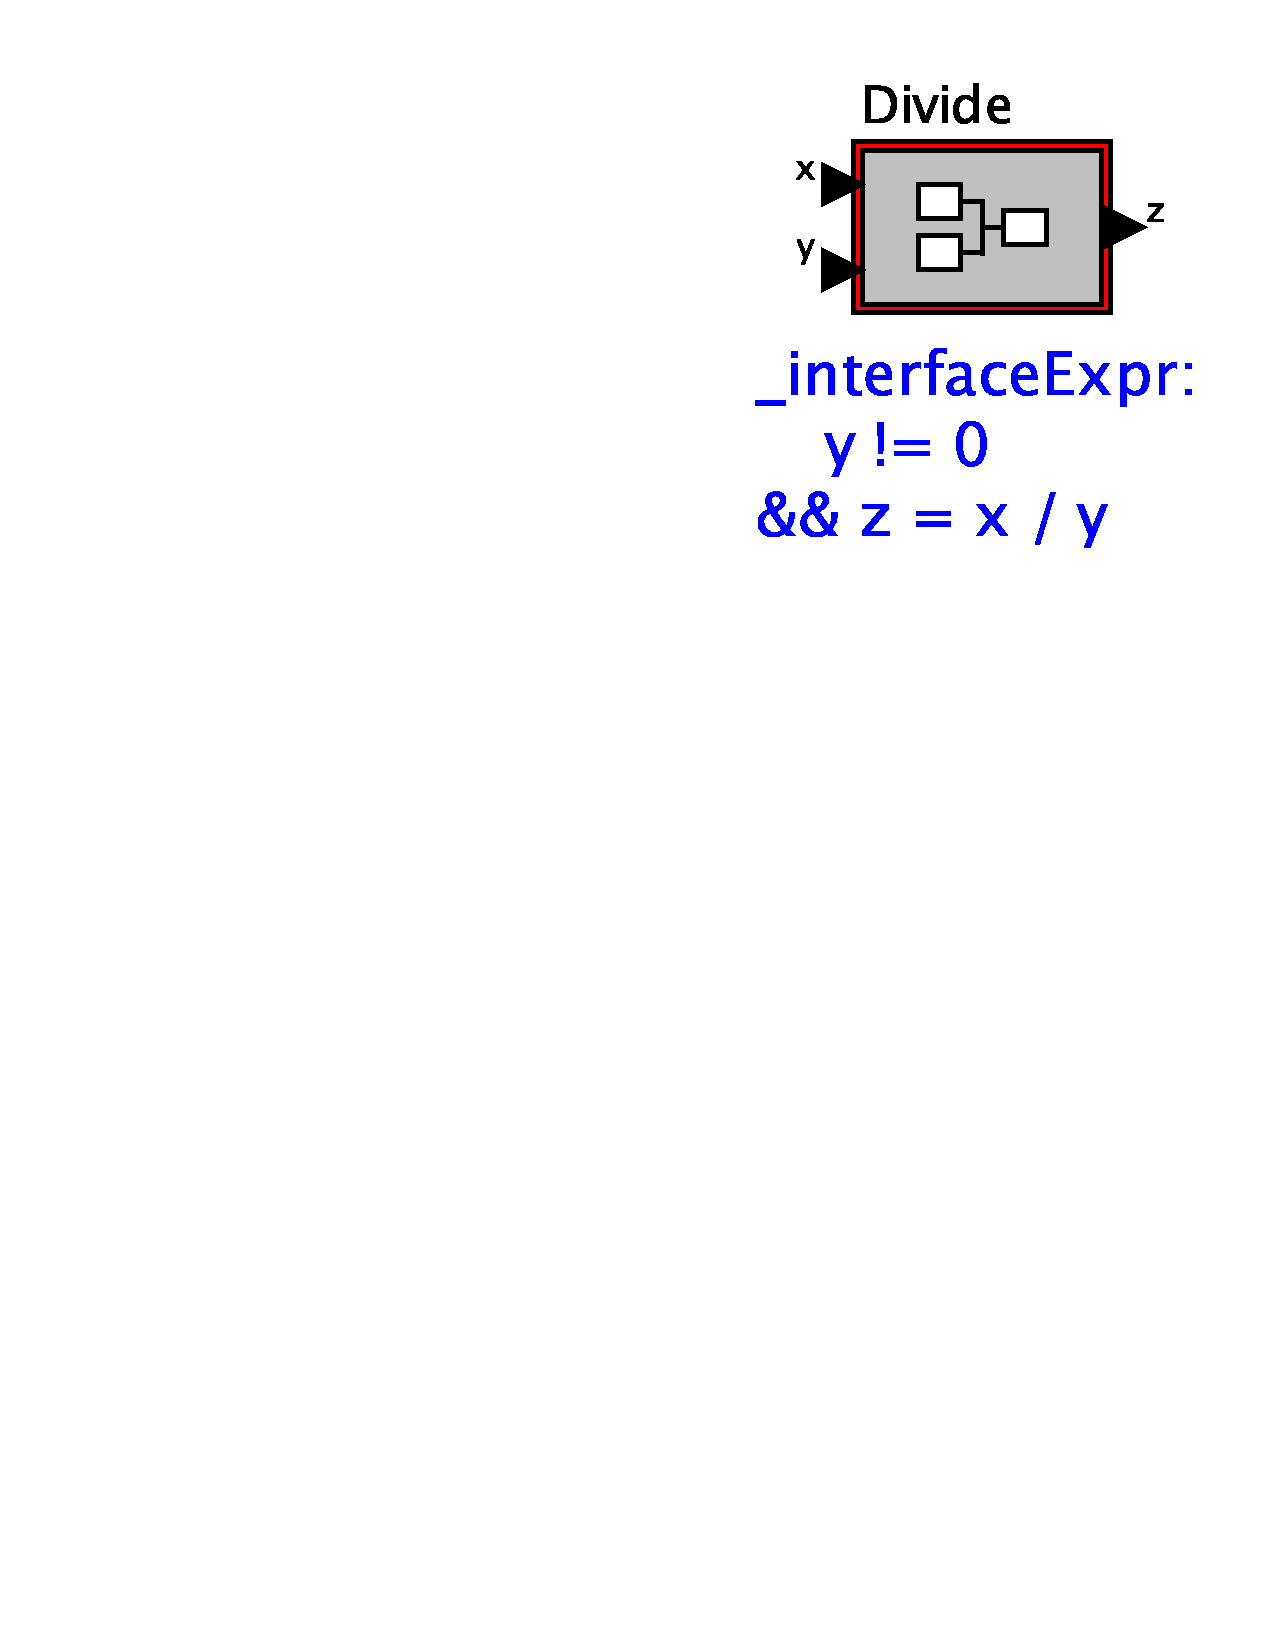
\includegraphics[scale=0.6]{figs/Divide2} % FIXME: Make old interface
\caption{A non-realtional interface of a divider actor.}
\label{fig:dividerOld}
\end{figure}

In a relational interface theory, however, we can express interfaces that are
more deterministic than this.  In fact, since this is a completely
deterministic component, whose behavior is uniquely determined by its (valid)
inputs, we can specify a completely deterministic interface.  We have shown how
this may look in Ptolemy in Figure~\ref{fig:dividerNew}, but it simply says
that the denominator must be non-zero, and the output is the quotient of the
numerator and the denominator.

\begin{figure}[htbp]
\centering
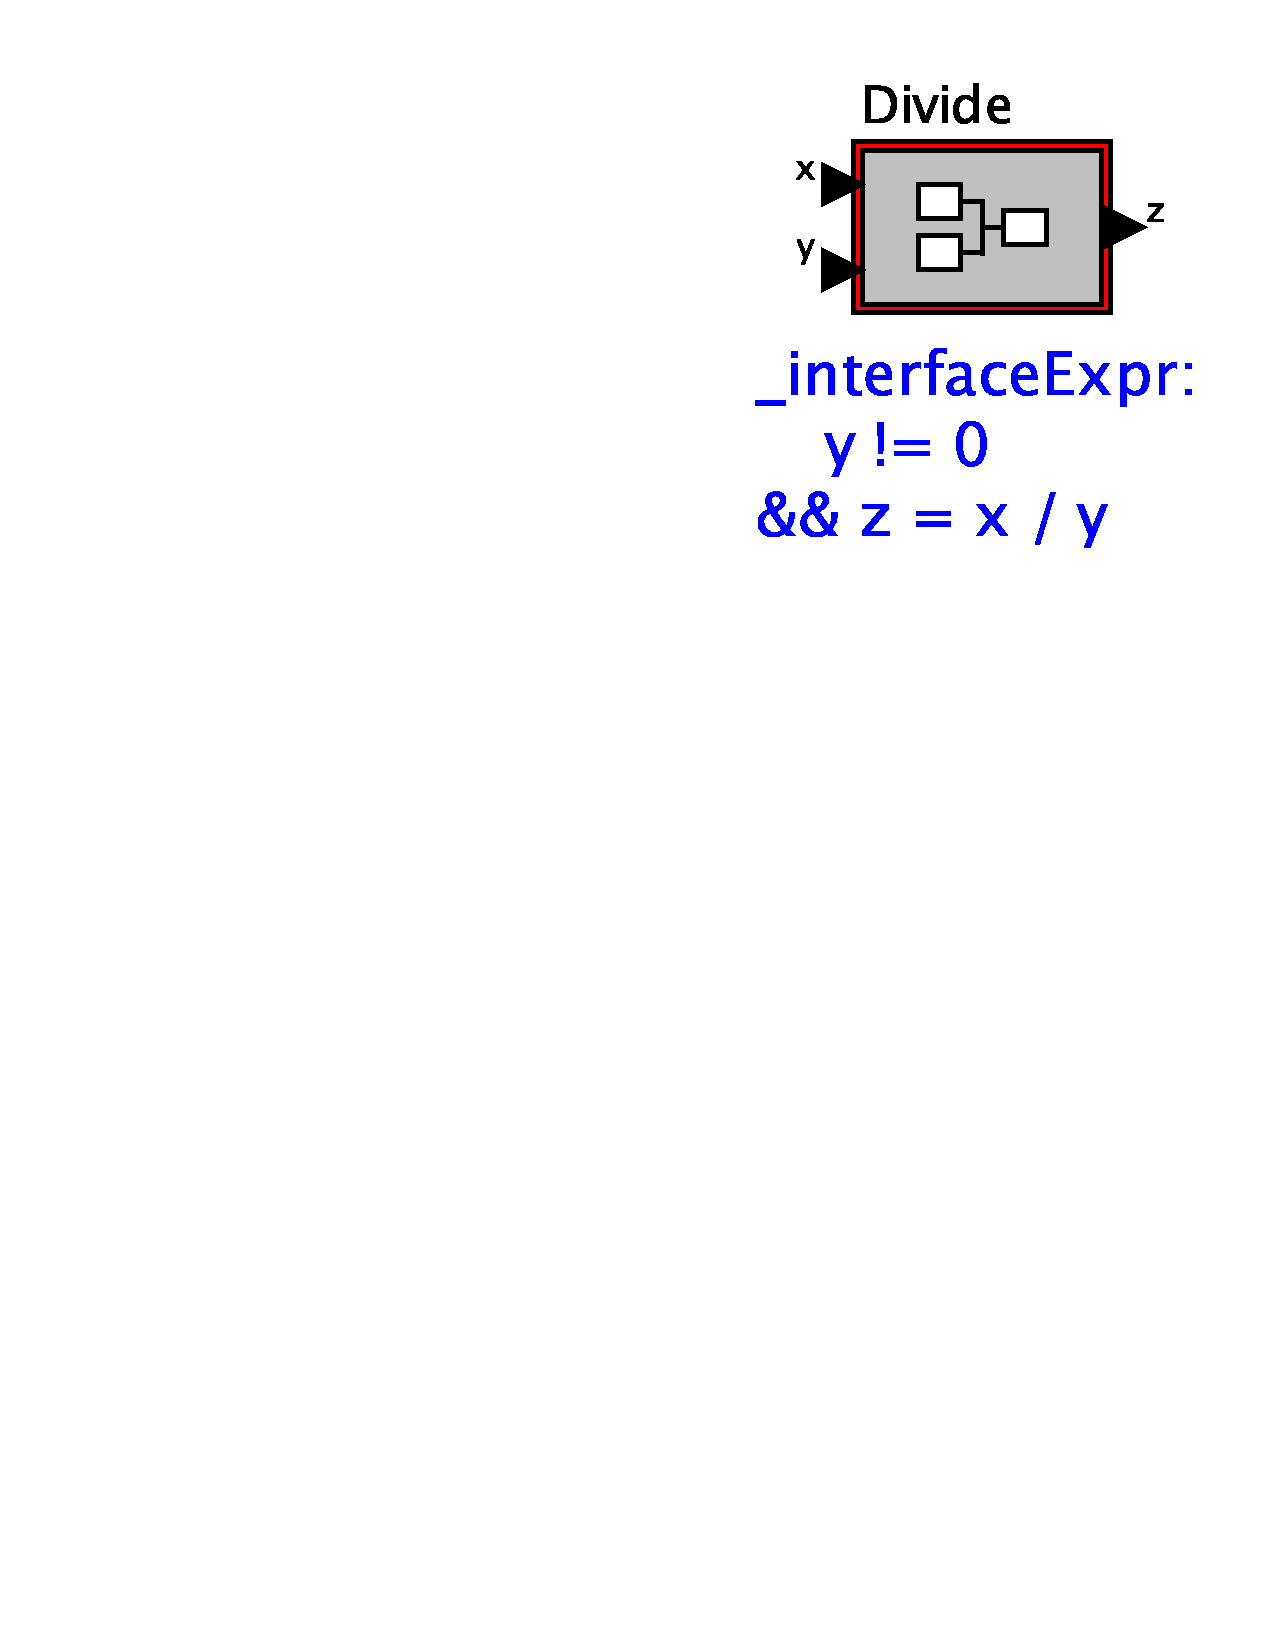
\includegraphics[scale=0.6]{figs/Divide2} 
\caption{A relational interface of a divider actor.}
\label{fig:dividerNew}
\end{figure}

Notice that if we want to recover the input assumptions, we can simply project
the contract onto the input variables by quantifying out the outputs.
In this case, the input assumptions are 
\[
\exists z : y \ne 0 \wedge z = x / y 
\]
This is equivalent to simply $y \ne 0$, which was exactly the input assumption
that we had previously.

\section{Solution}
Since there is ongoing research on creating industrial-grade SMT solvers,
we elect to integrate an existing solver rather than create one from scratch.
Our approach leverages the Yices\cite{yices} SMT solver, interfacing it to
work in the Ptolemy II\cite{ptII} modeling framework.

We do this through the use of a new Ptolemy~II director, called the
\texttt{InterfaceCheckerDirector}, which checks for the validity of interfaces
in the actors of a model. We allow each actor in the model to be annotated with
a parameter to specify its interface. Here we supporting both native Ptolemy~II
expressions, which have a C-like syntax, and LISP-style string expressions in
the Yices input language. The Ptolemy expressions must be boolean valued, with
a true value meaning the interface is satisfied, and they are searched for by
looking for parameters of actors named $\_interfaceExpr$. The Yices inputs
language interfaces require string-valued parameters names $\_interfaceStr$,
and allow richer expressions to be used. This is because the Yices input
language supports quantifiers, which are absent in the Ptolemy expression
language.

The details of the interface theory itself are encapsulated in the
\texttt{RelationalInterface} class, allowing for different interface theories
to be added later, although currently only the relational interface theory
of~\cite{relationalInterfaces} is supported. Interface theories themselves must
handle cascade composition from one interface to another, parallel composition
of two interfaces, and feedback composition. In cases where these compositions
are not possible, the interface theory must throw an exception.
%FIXME: Make this true

\subsection{Examples}
Here are some examples of how to use the tool to check for model compatibility.

In the first example, the user wants to compose two components.
In order to do that, he must first check that the interfaces are composable. 
The first component takes an absolute value, and the second component takes the
inverse of its input.

\subsubsection{Interface Error}
\begin{figure}[htbp]
\centering
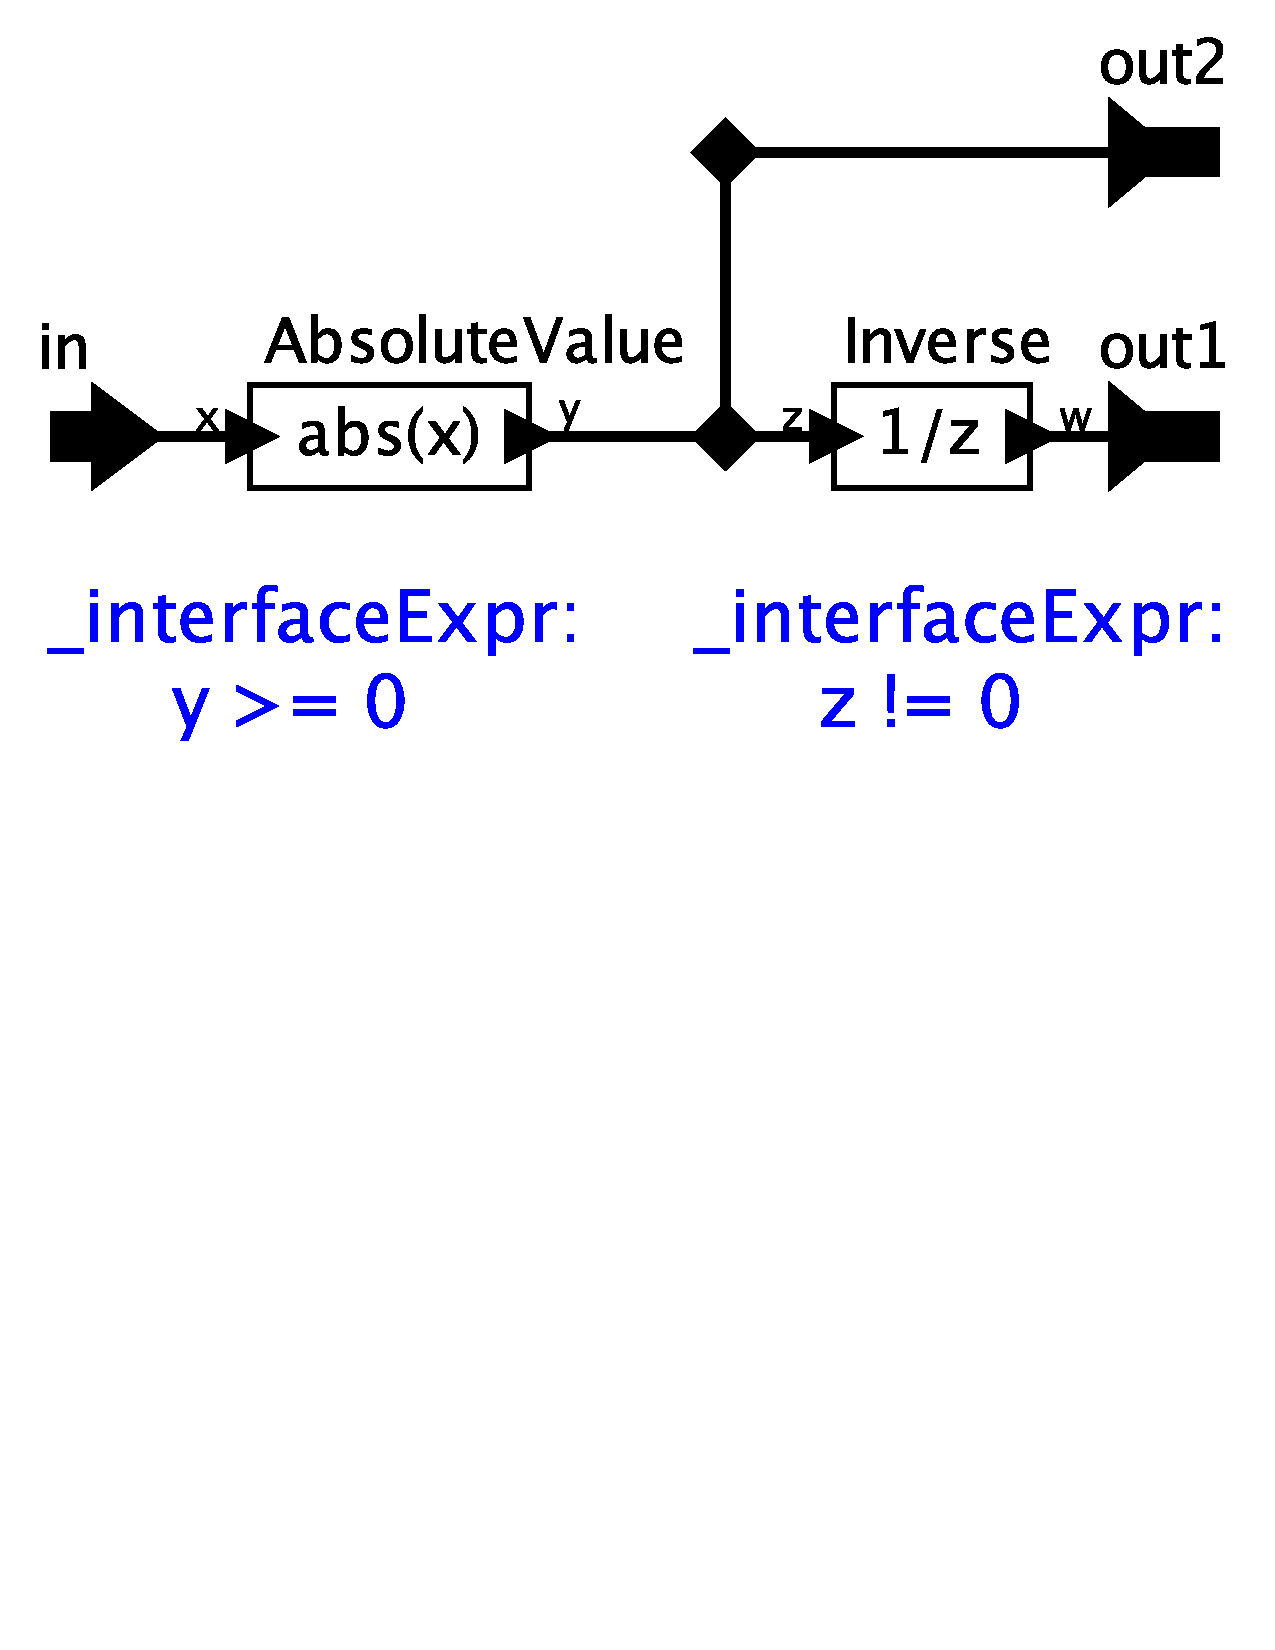
\includegraphics[width=\columnwidth]{figs/absoluteError}
\caption{An error in interface specification.}
\label{fig:absoluteError}
\end{figure}

In this example, interfaces are being used to prove safety properties of the
system, so any abstractions must be overapproximations.
In the first attempt, the user choses the contract
\[
y \ge 0
\]
for the absolute value.
<!--If we consider this formula as a relation,
it contains all pairs of inputs and outputs such that
the input is not simultaneously zero with the output non-zero.-->
Clearly this is an overapproximation of absolute value, since it doesn't take
into account the input to the actor. For the inverter, the user choses the
contract
\[
x \ne 0
\]
to capture the restriction that we cannot divide by zero.
Since this contract does not specify the output value, it too is an abstraction
that overapproximates.

\begin{figure}[htbp]
\centering
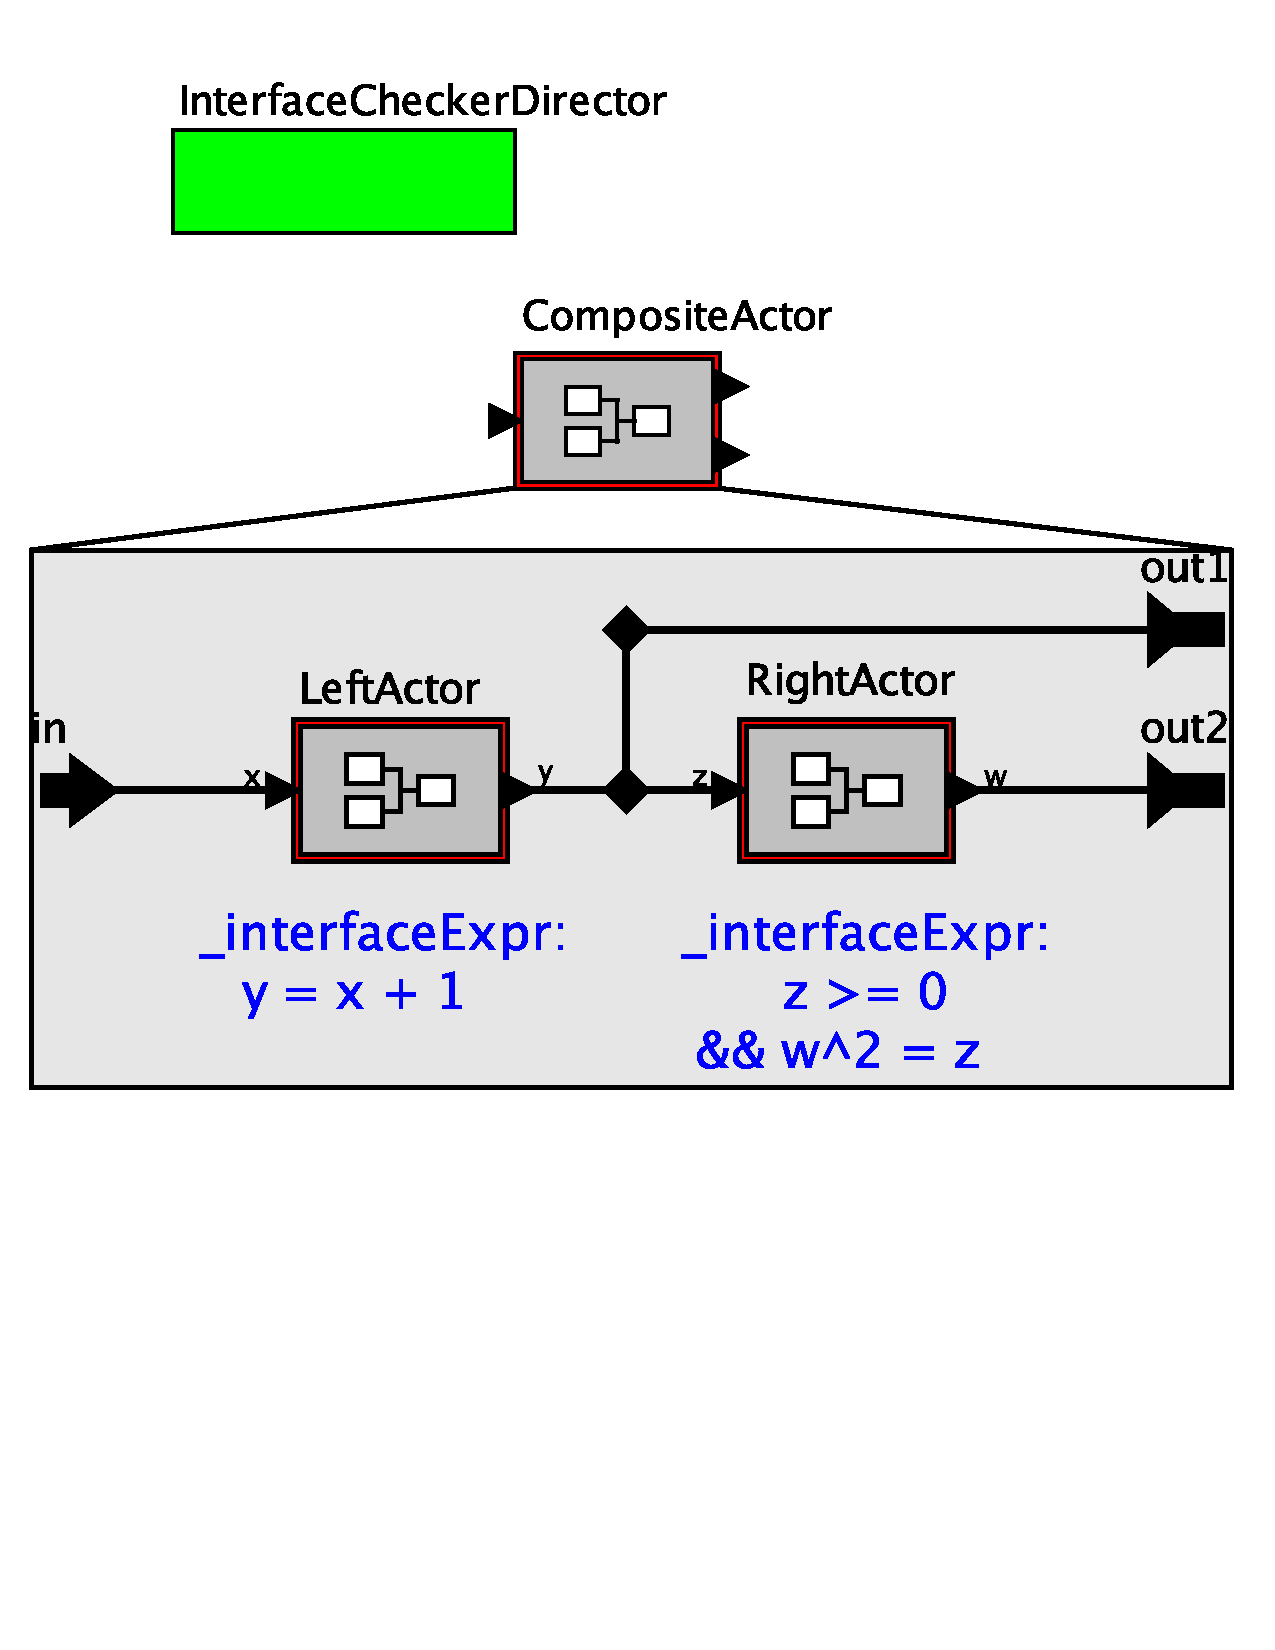
\includegraphics[width=\columnwidth]{figs/cascadeComp} 
\caption{A composite actor formed by the cascade composition of two contained
actors.}
\label{fig:cascadeComp}
\end{figure}

\begin{figure}[htbp]
\centering
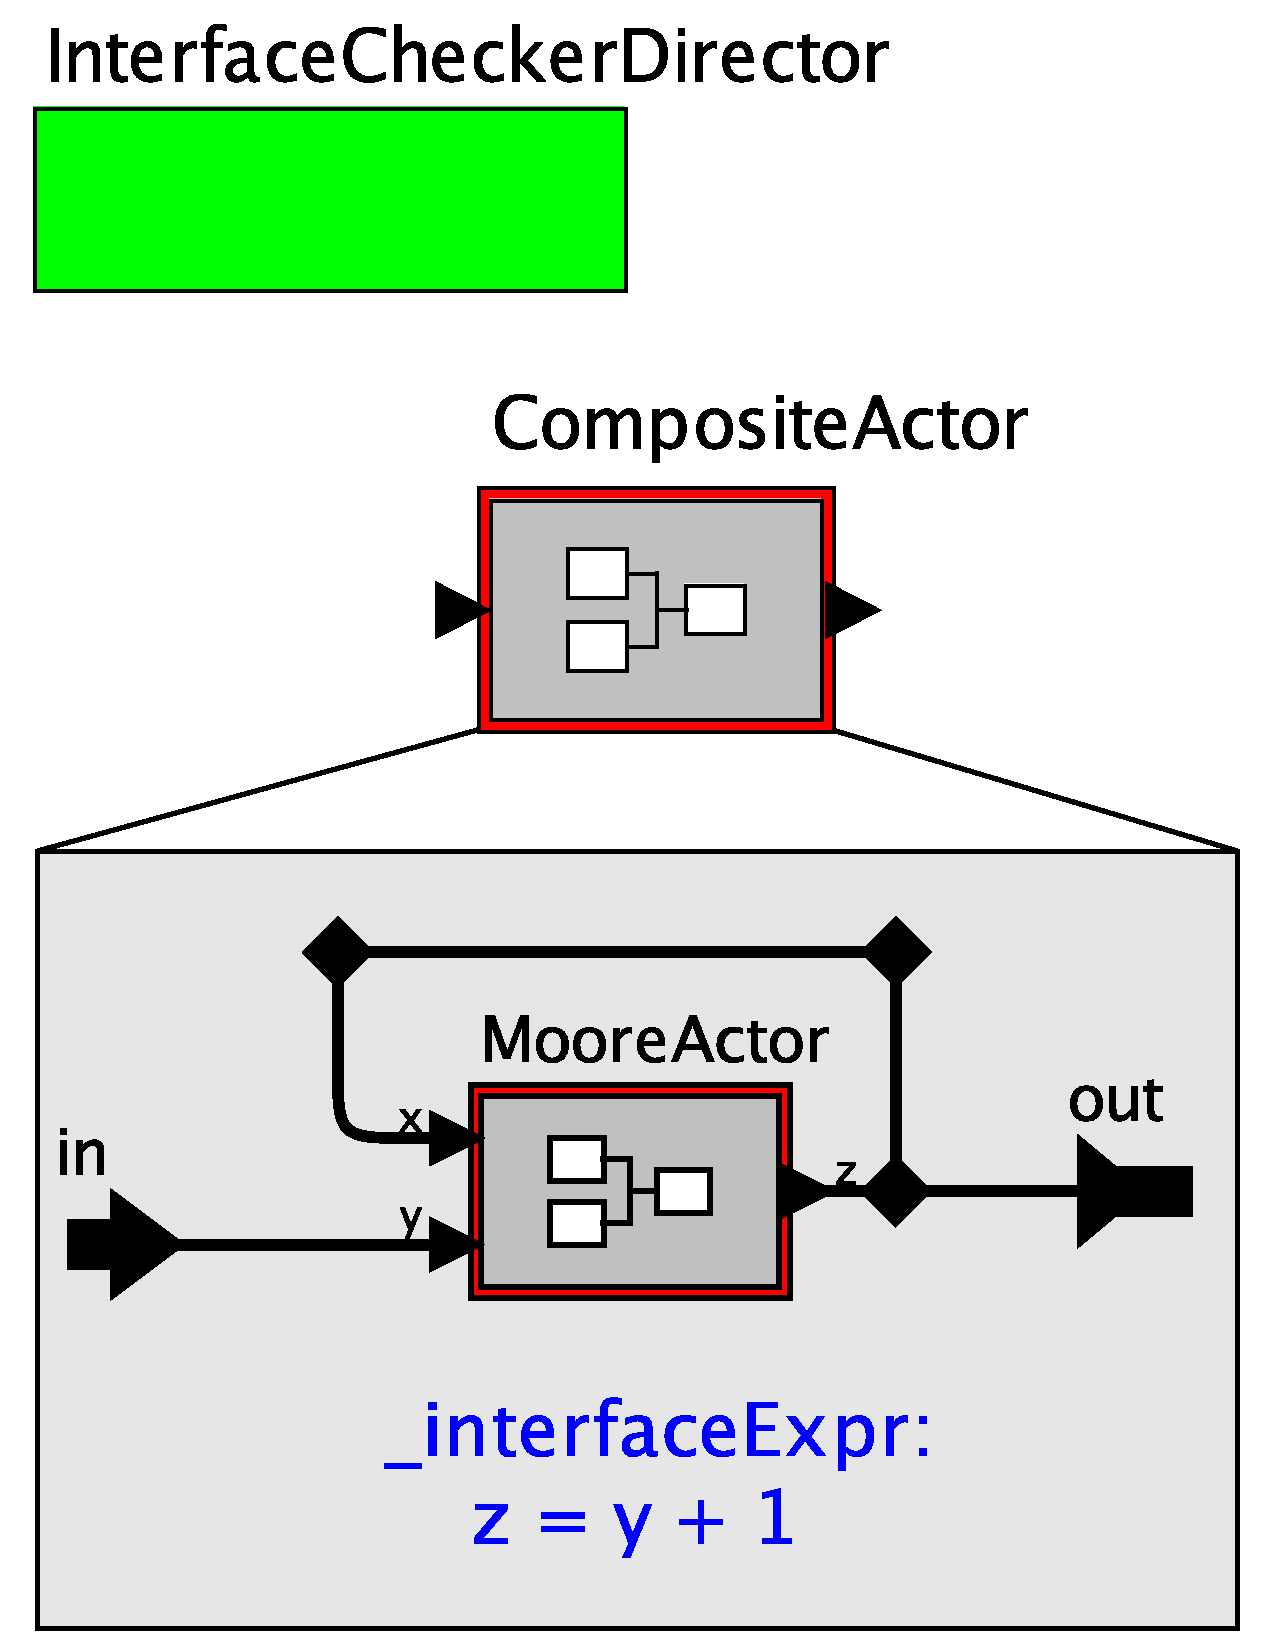
\includegraphics[width=\columnwidth]{figs/feedbackComp} 
\caption{A composite actor formed by adding feedback to its contained actor.}
\label{fig:feedbackComp}
\end{figure}

In this case, if we run our tool, we can see that the resulting composition
interface is not valid.
Intuitively, this is because there is no input to the first interface such
that we can guarantee its output will not be zero.
Since these interfaces do not compose, we need to make them more concrete.

\begin{figure}[htbp]
\centering
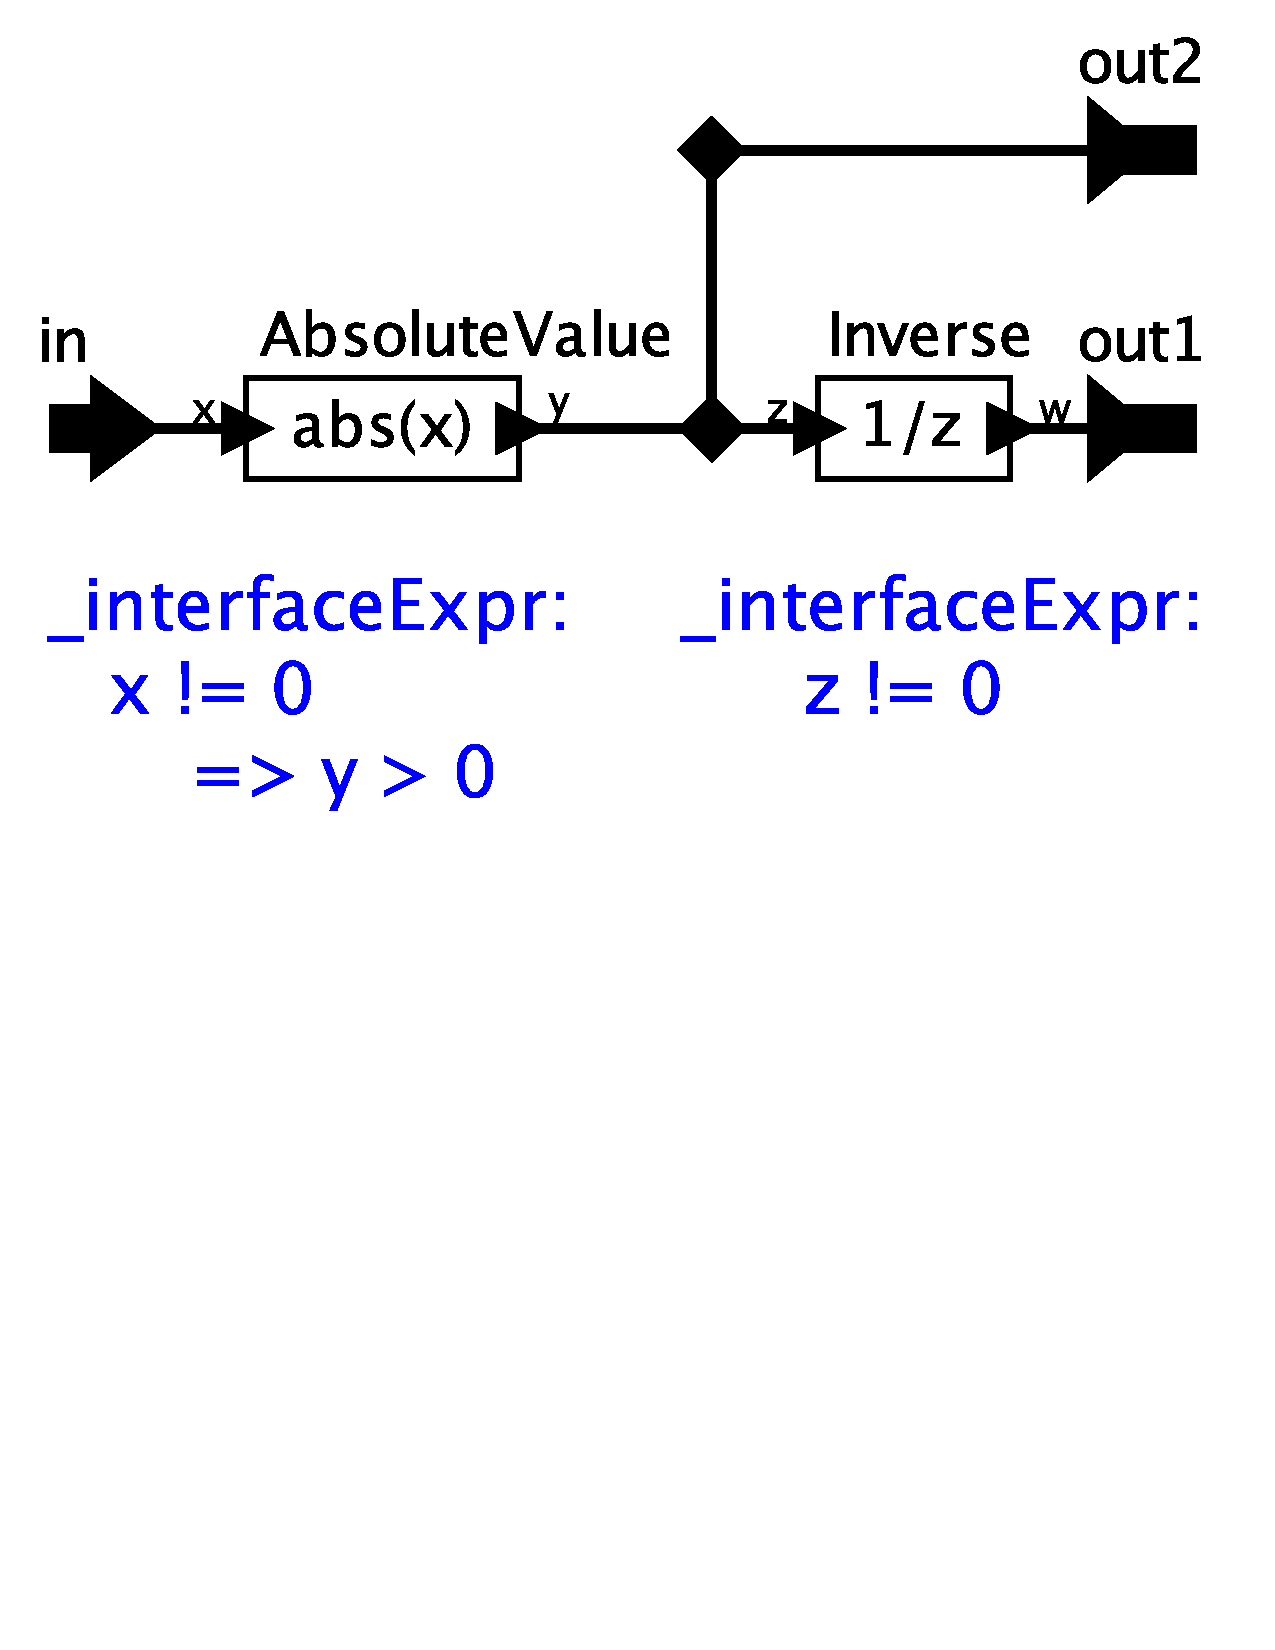
\includegraphics[width=\columnwidth]{figs/absoluteCorrected}
\caption{A fixed interface specification.}
\label{fig:absoluteCorrected}
\end{figure}

A second attempt at defining the component interfaces for this same model is
given in Figure~\ref{fig:absoluteError}.
Here, the interface of the inverter is unchanged,
but the interface for the absolute value is changed to
\[
a \ne 0 \implies y > 0
\]
P.S. Let's try an example with \[ a \ge 0 \implies y = a\] or even \[a \ge 0
\implies y = a  \wedge a < 0 \implies y = -a\]

\subsubsection{Component Error} \label{sec:componentError}
\begin{figure}[htbp]
\centering
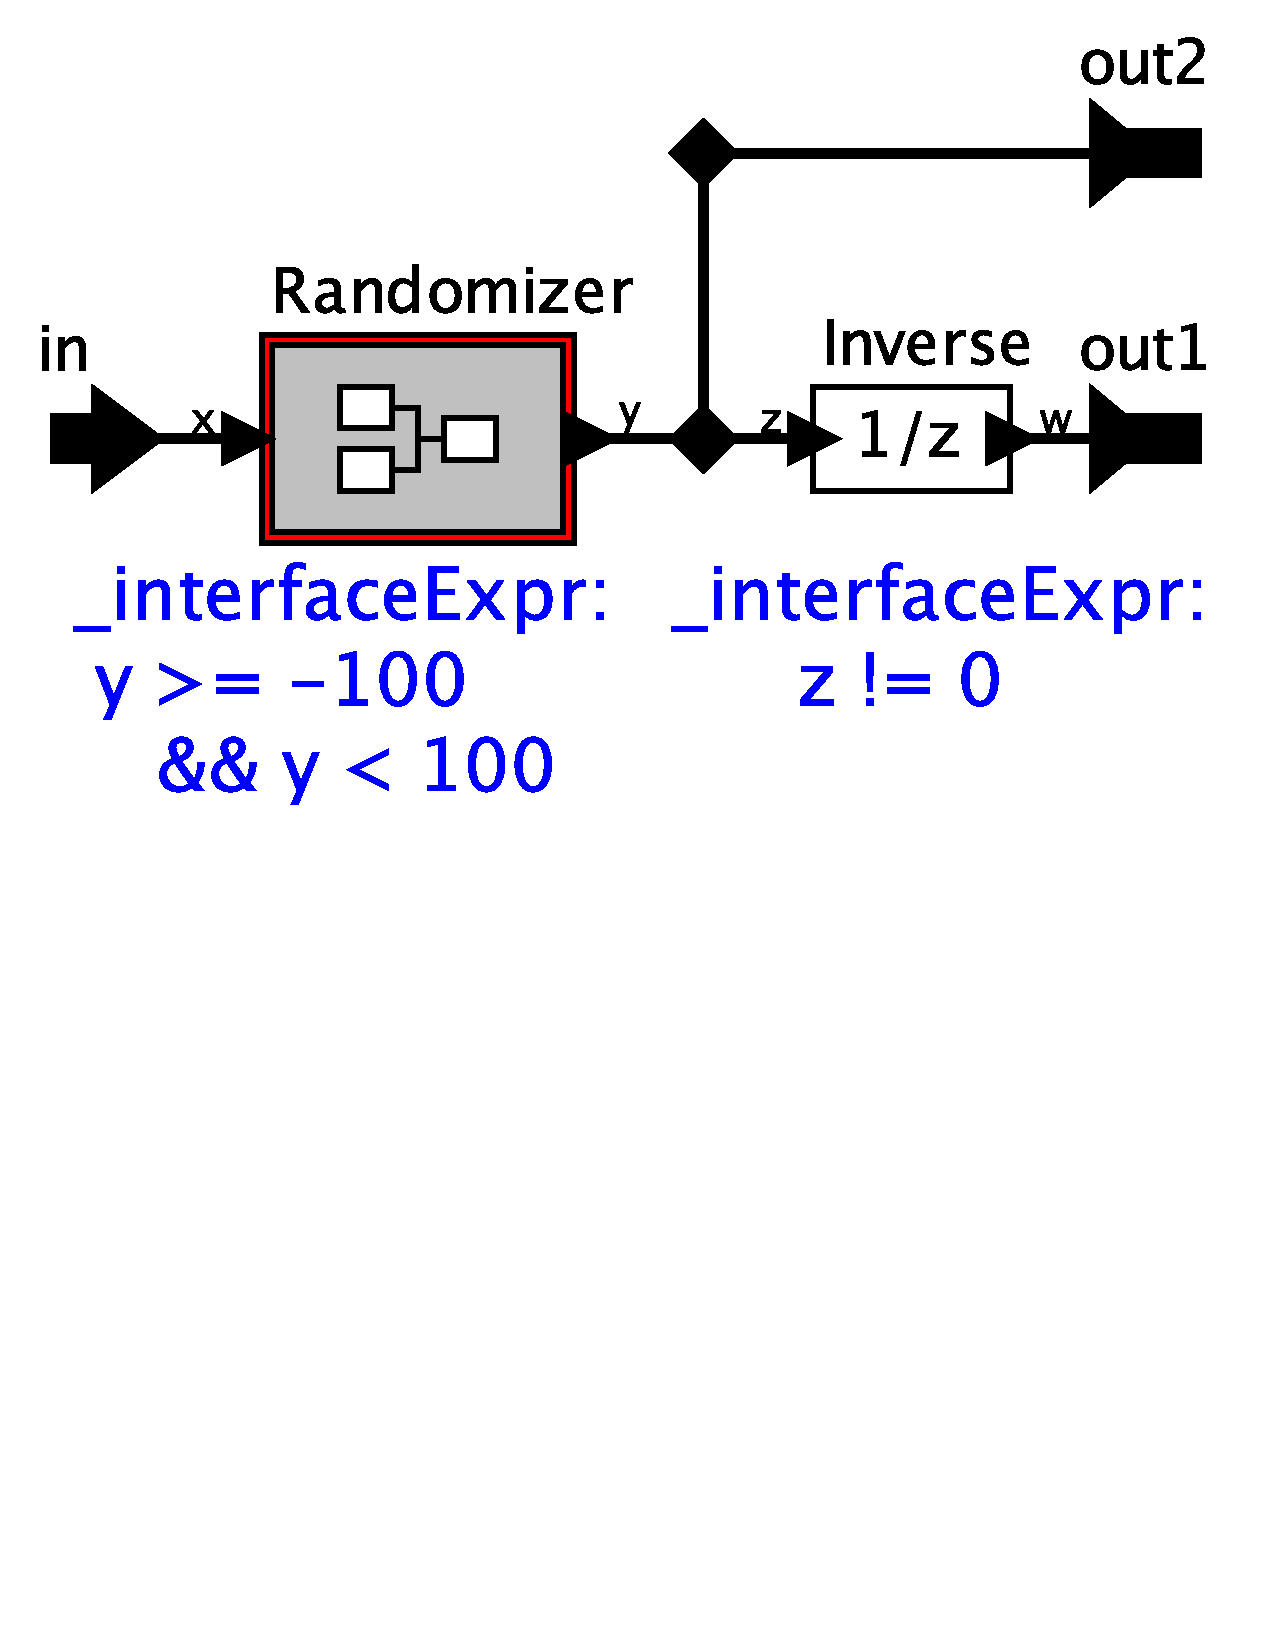
\includegraphics[width=\columnwidth]{figs/Randomizer}
\caption{An error in component composition.}
\label{fig:randomError}
\end{figure}

Consider another example in which the first component produces a random value
in the range $[2^{-31}, 2^{31}-1]$, and the second component is the same as
before.
The most deterministic valid constraint that the user can use for the first
component would be
\[
y \ge 2^{-31} \wedge y \le 2^{31}-1
\]

In this case, running our tool will tell us that these components cannot be
composed.
This time, however, this is not caused by the interfaces being too abstract;
in fact, they are maximally deterministic.
The reason why we cannot compose these interfaces is that these components
cannot be safely composed.

\section{Ongoing work}
As a general infrastructure, there are many possible extensions.
One would be the addition of run-time checks to test that the values produced
by the implementation conform to the interfaces. This could be a check of both
the implementations and the interfaces. Interestingly, these checks could even
have predictive power. As an example, consider Figure~\ref{fig:randomJitter}.
Here, the first component adds a value to its input that is randomly chosen
from the range $[-100,100)$. Since there is non-determinism in the component,
the given interface, $x-100 \le y < x+100$, is as deterministic as possible.
Unlike the totally random component from Figure~\ref{fig:randomError}, these
components can be validly composed by restricting the acceptable inputs $x$
that can be provided to the composite. In isolation, static analysis on this
component will declare it to be error-free. \begin{figure}[htbp]
\centering
\includegraphics[width=\columnwidth]%{figs/randomJitter}
{figs/Randomizer} %FIXME: Add random jitter screenshot
\caption{A component with an error that may not show up through testing.}
\label{fig:randomJitter}
\end{figure}
Imagine that we had test cases that ran this code with an input of $42$.
This would be an erroneous composition, since running the model could cause
the first component to output $0$, resulting in a divide by zero error.
Through standard testing, however, the odds of finding this error by running
the model would be very small ($0.5\%$, in this example). If we used run-time
checks of our interfaces, however, then we could detect unsafe uses through
testing, and always flag a test case with an input of $42$ as violating the
input requirements of the composite interface. Then any run using a value
within the jitter of zero would be flagged as incompatible, even if that
particular run caused no error in any component.

The interface theory also defines a notion of one interface \emph{refining}
another, which simply means that refining interface can be used in place of the
refined interface in any environment.
Formally, the definition is that $I'$ refines $I$ if the following two
conditions hold:
\begin{align*}
in(\phi) \implies in(\phi') \\
in(\phi) \wedge \phi' \implies \phi
\end{align*}
where $\phi$ and $\phi'$ are the contracts of $I$ and $I'$ respectively, and
$in(\phi)$ gives the input assumptions for the contract by projecting onto the
input variables.

It would be useful to allow model builders to check that one model
refined another.  One concrete use case would be in comparing the
inferred interface of a composite actor to a desired interface given by the
model builder.  If the inferred interface does not refine the given interface,
then there exists a modeling error.  This is because this would mean that the
composition of interfaces allows some behavior that the desired interface did
not.
%
This can also be checked algorithmically by an SMT solver, by simply checking
that the conjunction on conditions of refinement between the two interfaces is
a tautology.  As an additional benefit, the SMT solver could produce a
counterexample, consisting of trace of the components that does conform to the
composite specification.

\section{Conclusion}
Here, we have presented an infrastructure for verifying interfaces of
components in Ptolemy~II, our actor based modeling tool. Our work
allows users to annotate Ptolemy II models with interface specifications in a
variety of formats, without changing the execution semantics of the model.
We also support automatically checking the validity of interface, as well as the
compatibility of interfaces for composition, and work on checking refienment
and run-time conformance is in progress. In addition, our work is the first to
present a general infrastructure for interfaces in Ptolemy~II.

There are many possible, more long term extensions to this work. There are
likely situations where users would prefer to see in inferred interface,
rather than simply make queries on it.  In the current tool, while they can
view inferred interfaces, they are not simplified, and often too complicated to
be easily understood.  Existing tools, such as QEPCAD~\cite{qepcad}, can
simplify logical formulas and remove quantifiers, and could likely help here.
Other possible extensions include observing behavior of components that have no
specified or inferrable interfaces, and guessing and learning potential
interfaces; or checking statically that the Java definition of an atomic actor
does not violate its interface.

Finally, one of the most important uses of this tool is for developing new
interface theories. Using this tool allows for rapid experiment with various
interfaces, storage of examples in an executable form, and checking of hand
proved results. In addition, the architecture encourages swapping out of one
interface theory for another, which intends to make it easy to experiment with
new theories altogether.

\acks

Acknowledgments, if needed.

% We recommend abbrvnat bibliography style.

\bibliographystyle{abbrvnat}
\bibliography{refs}

\end{document}
